\chapter{Experiments} \label{chapter:experiments}

The following section describes the setups of the experiments conducted with the neural network presented in Chapter \ref{chapter:semi_automatic}. Due to the lack of existing annotated medical data the focus of the experiments is to ascertain a network design and mode of operation that compensate this as best as possible. First, we test the different network architectures that were described in section \ref{section:network_variations} using the same parameters. We then choose the best architecture for further experiments, in which we evaluate the two different training schemes introduced in section \ref{section:modes_of_operation}: training from scratch and incremental training.

\section{Terminology}

\noindent\textbf{Hyper-Parameter.} \textit{Hyper-parameters} are the tunable parameters of a network. The number and kind of parameters varies with the used type of network architecture, optimizer, etc.

\section{Datasets}

\begin{figure}[!tbp]
	\centering
	\begin{subfigure}[t]{0.47\textwidth}
		\centering
    	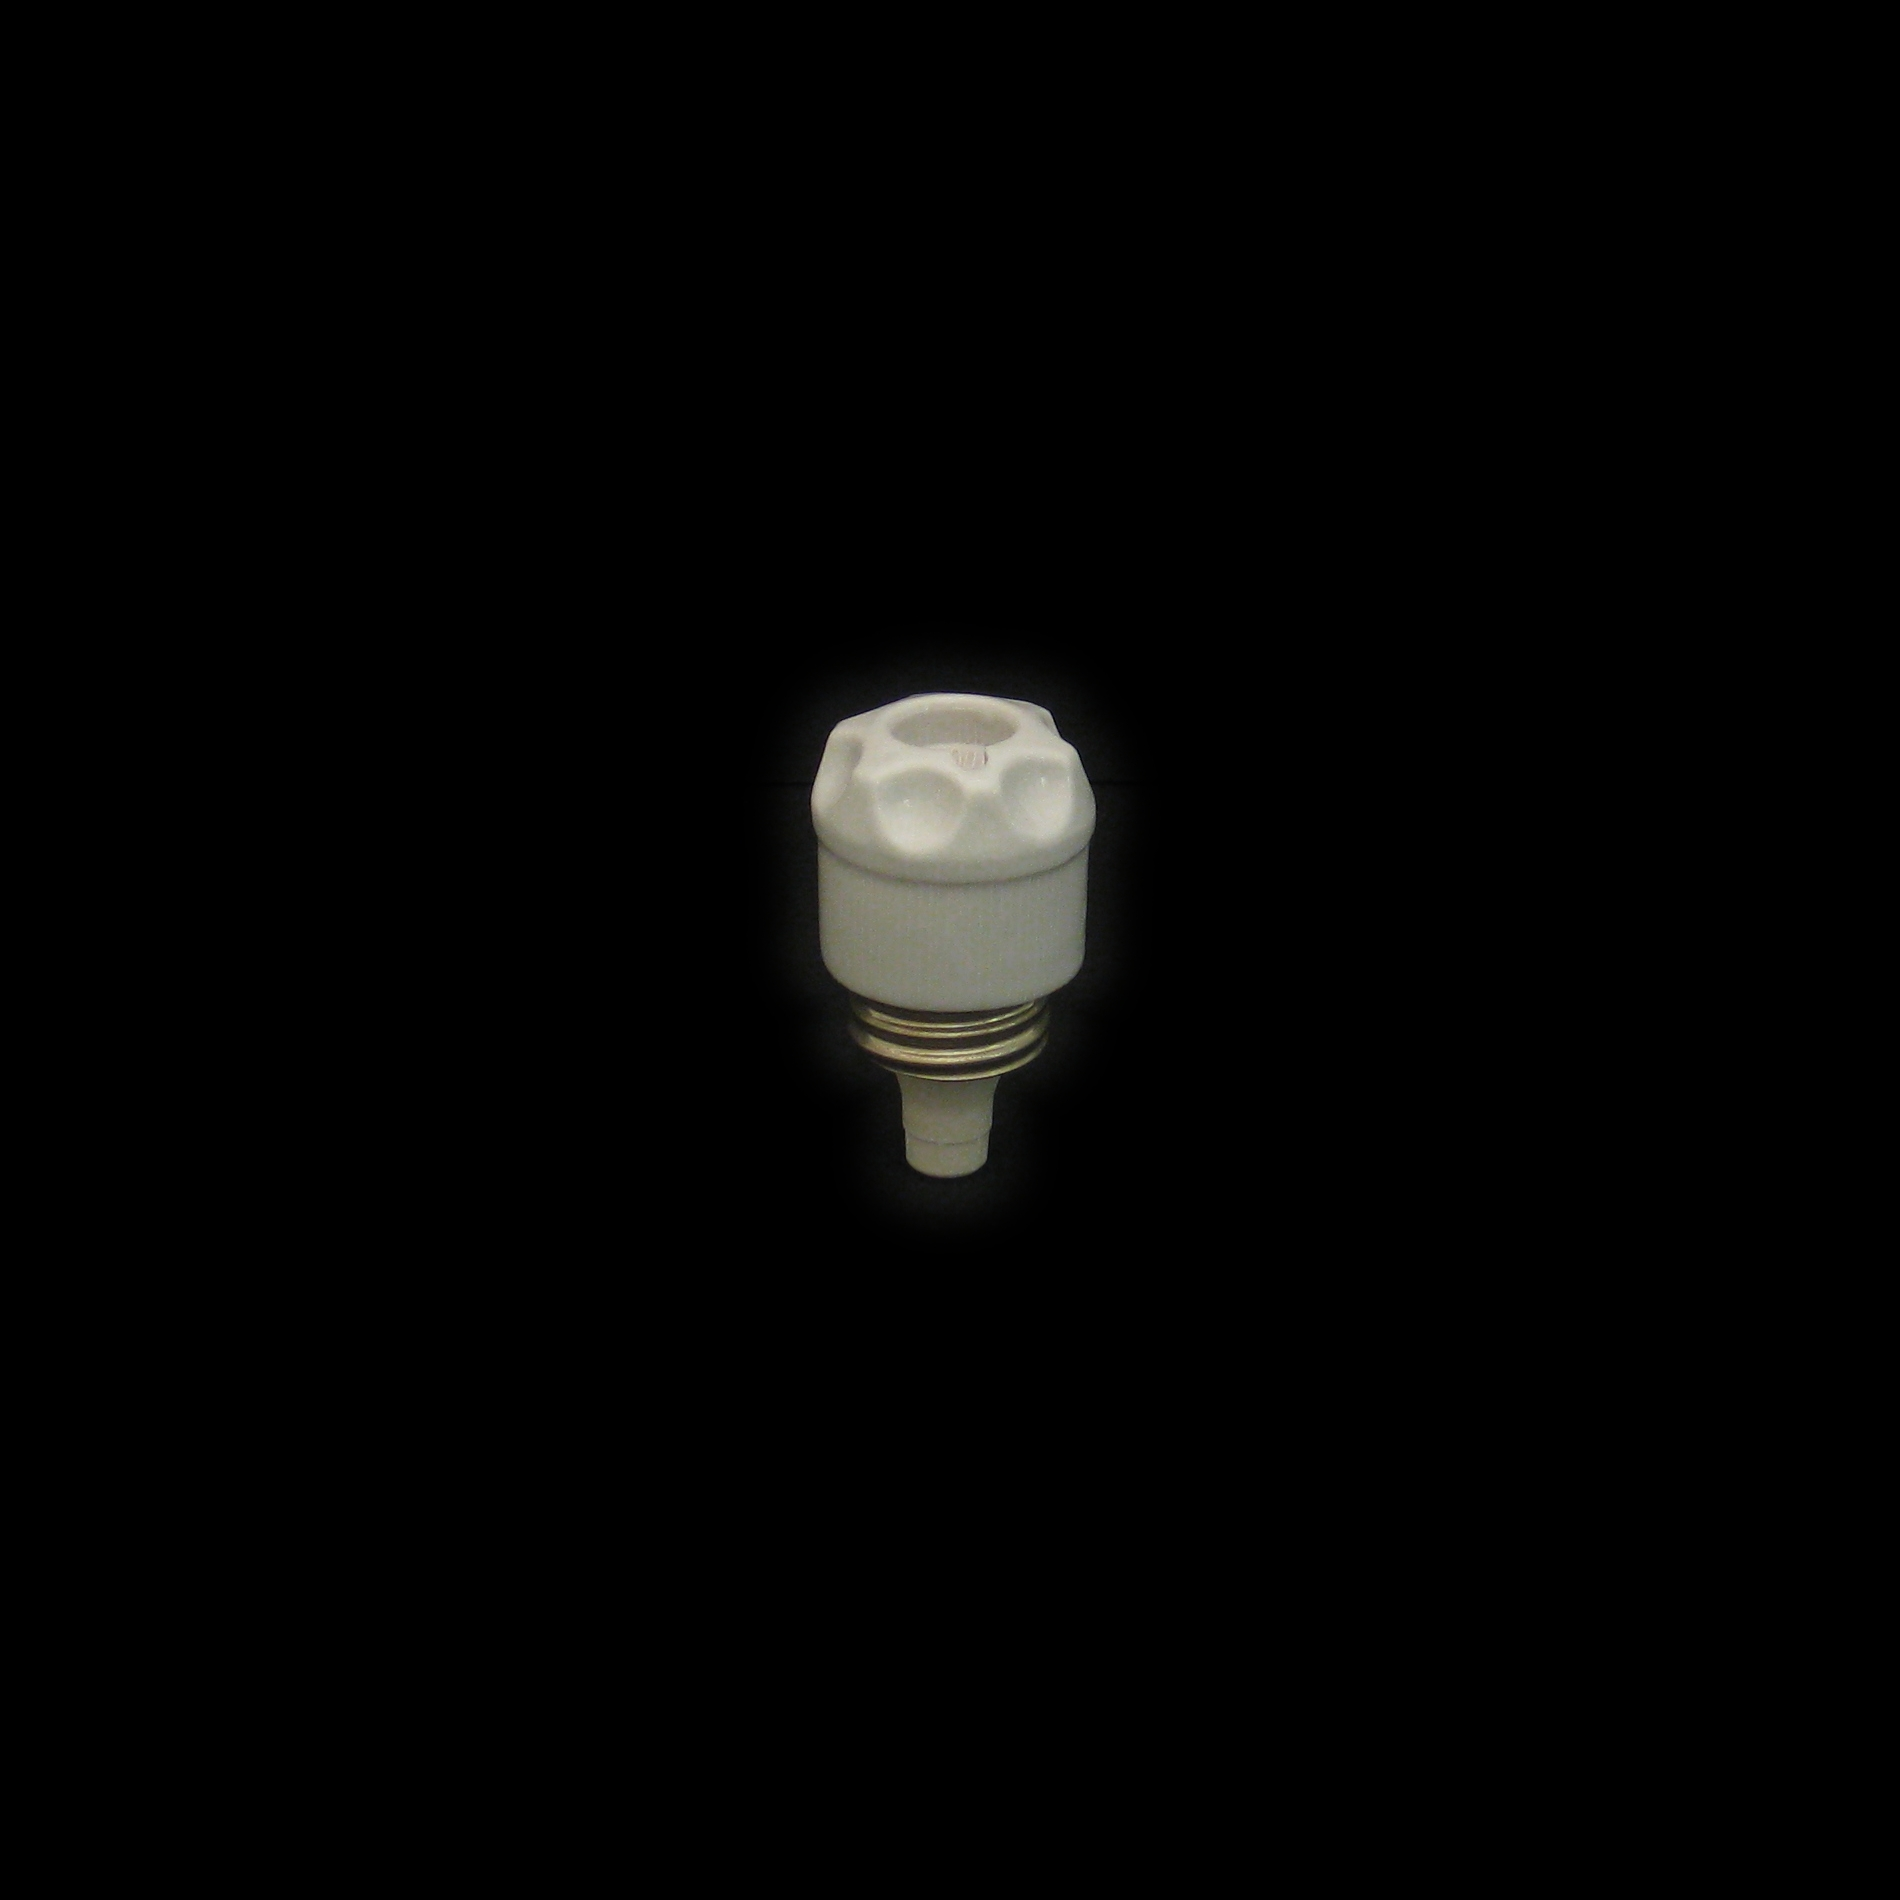
\includegraphics[width=0.6\linewidth]{tless_example_train}
    	\caption{An example frame from the training dataset of T-Less.}
    	\label{fig:tless_example_train}
	\end{subfigure}
	\hfill
	\begin{subfigure}[t]{0.47\textwidth}
		\centering
    	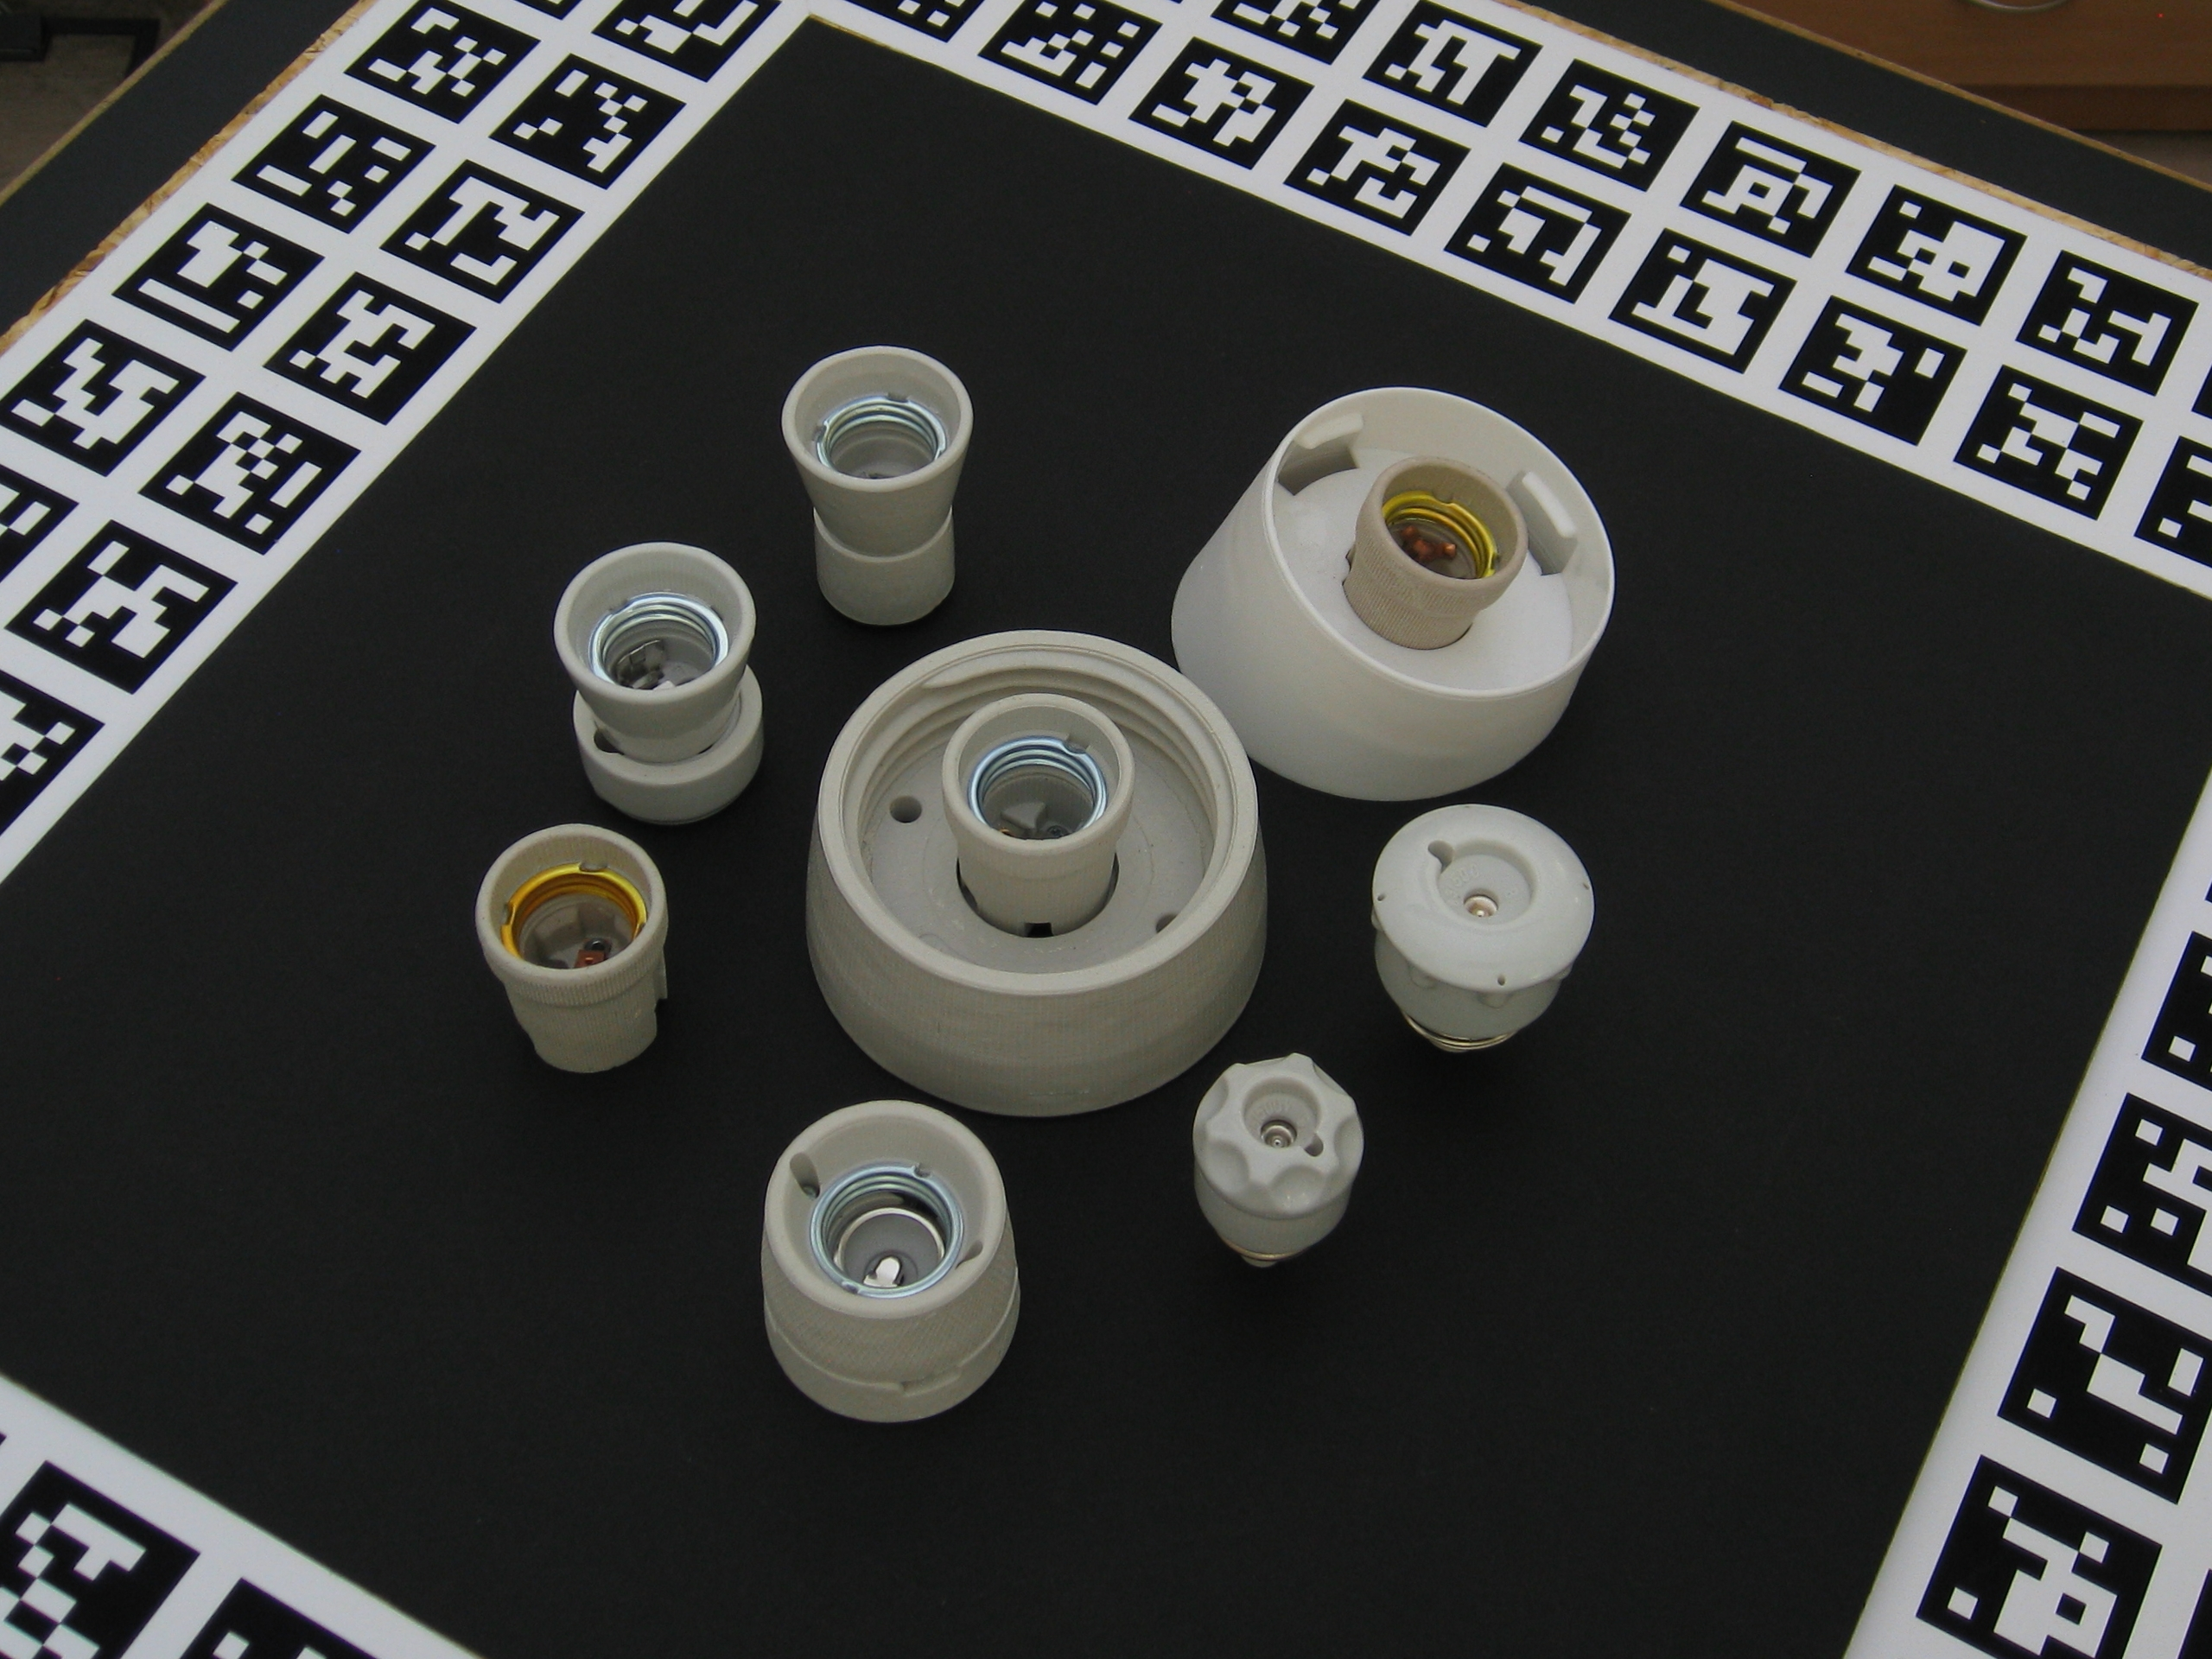
\includegraphics[width=0.7\linewidth]{tless_example_test}
    	\caption{An example frame from the test dataset of T-Less.}
    	\label{fig:tless_example_test}
	\end{subfigure}
	\caption{Example frames from the T-Less dataset \cite{tless}.}
	\label{fig:tless_examples}
\end{figure}

The initial intention to completely annotate the medical images provided at the beginning of the project turned out to be not feasible (see Chapter \ref{chapter:manual_annotation}). Instead, we chose the T-Less dataset to conduct the experiments with. Its objects are mostly texture-less  and of rather small size making them similar to surgical tools. Next to many human pose estimation datasets, there exist some datasets of objects too, like \cite{next_view_dataset}, \cite{pracsys_dataset} and \cite{rigid_body_dataset}. But the objects of T-Less resemble surgical tools more than the objects of those datasets.

The T-Less dataset was released in 2017 by Hoda\v{n} et al. \cite{tless}. It contains the object models of 30 industry-relevant real world objects. Two versions exist: one mesh of the object that was manually reconstructed using CAD software and one that was produced from RGB-D images. The 3D coordinates of the objects reflect their size in millimeters. For example, the minimum and maximum of any component of the coordinates of object model 01 are about -30 and 30. This means that the model is about 60 mm or 6 cm long. The objects were captured using a Primsense CARMINE 1.09, a Microsoft Kinect v2 and a Canon IXUS 950 IS. We used the photos of the Canon camera due to their quality and we do not need depth information, which is also provided by the CARMINE sensor and the Kinect. There are 1296 images of each object in the training set of the dataset, sampled in 10 degree steps in elevation and 5 degree azimuth. 20 test scenes, consisting of 504 images each, exist as well. Those are photographs of cluttered scenes of different complexity, with sometimes more than 15 objects visible. All training and test images are annotated with the ground-truth poses of the visible objects. The authors also provided a tool set to render the objects at a given pose, etc. Fig. \ref{fig:tless_example_train} shows an example frame from the training set and fig. \ref{fig:tless_example_test} an example frame from the test set. The training images of the other objects look similar to the one shown. The dataset provides depth images, as well, but this is irrelevant to our setting.

%TODO network predicts coordinates for all pixels belgongin to the segmentation mask -> special handling necessary but not implemented when multiple instances of the object are visible

\section{Data Preparation}

The \textit{T-Less} dataset does neither provide 3D object coordinates nor segmentation masks. This is the reason why we rendered both ourselves. The script is part of the network package. Because the 16-bit TIFF object coordinate ground-truth files used up too much disk space when in original size they were cropped to the relevant area by determining the smallest box around the segmentation pixels. The images and segmentation masks were cropped to the same area and the camera matrices adjusted accordingly. We used 16-bit TIFF files instead of 32-bit because we deemed the accuracy of 16-bit enough.

\section{Metric}

We developed a set of evaluation metrics to capture different aspects of the prediction quality of a network. We assumed that multiple metrics provide better insights of the strengths and weaknesses of an architecture. To this end, we provide functionality that directly assesses the quality of the predicted object coordinates and also functionality that provides details on the accuracy of the resulting recovered pose.

The \textit{Object Coordinate Error} $e_{\text{coord}}$ computes the euclidean distances between the predicted and ground-truth object coordinates
\begin{align*}
e_{\text{coord}} = \frac{1}{|S_O|} \sum\limits_{(i, j)} \sqrt{(g_{ij1} - p_{ij1})^2 +(g_{ij2} - p_{ij2})^2 + (g_{ij3} - p_{ij3})^2}
\end{align*}
where $(i, j)$ are all 2D locations belonging to the object model $O$ according to the segmentation mask. $|S_O|$ denotes the cardinality of the set of these locations. $g_{ijk}$ and $p_{ijk}$ are the $k$-th components of the object coordinate at $(i, j)$ in the ground-truth and predicted object coordinates image, respectively.

The number of \textit{Inliers} $n_{\text{inlier}}$ captures the number of object coordinates whose euclidean distance to the ground-truth object coordinate is below a threshold:
\begin{align*}
e_{\text{inlier}} = \left\rvert\left\lbrace(i,j) \ \bigg| \ \sqrt{(g_{ij1} - p_{ij1})^2 +(g_{ij2} - p_{ij2})^2 + (g_{ij3} - p_{ij3})^2} \leq \sigma_{\text{thresh}}\right\rbrace \right\rvert
\end{align*}
where $\sigma_{\text{thresh}}$ is the chosen threshold and $(i,j)$ are again all locations belonging to the object model. We set the threshold to 2.

Both $e_{\text{coord}}$ and $n_{\text{inlier}}$ assess the accuracy of the predicted object coordinates. The metrics described next provide a measure of the quality of the recovered pose.

The \textit{Distance Error} $e_{\text{dist}}$ is the euclidean distance between the ground-truth position of the object and the position computed by \ac{ransac} by solving the \ac{pnp} problem. $e_{\text{dist}}$ is computed as
\begin{align*}
e_{\text{dist}} = \sqrt{(t_{g1} - t_{p1})^2 +(t_{g2} - t_{p2})^2 + (t_{g3} - t_{p3})^2}
\end{align*}
where $t_{gk}$ denotes the $k$-th component of the ground-truth translation vector, and $t_{pk}$ the $k$-th component of the translation vector recovered from the coordinate predictions.

The \textit{Angle Error} $e_{\text{angle}}$ is the rotational error in degrees between the ground-truth and calculated rotation matrix
\begin{align*}
e_{\text{angle}} = \frac{cos^{-1}(\frac{\Tr(R_g^TR_p) - 1}{2}) \cdot 180\degree}{\pi}
\end{align*}
where $R_g$ and $R_p$ denote the ground-truth and predicted rotation matrix, respectively and $Tr()$ denotes the trace of a matrix.

Finally, we also implemented the metric presented by Hinterstoisser \etal in \cite{hinterstoisser2}, which computes the average distance between each vertex of the object model with the ground-truth and recovered pose applied to it. This metric $e_{\text{pose}}$ is defined in the following way
\begin{align*}
e_{\text{pose}} = \frac{1}{|M|} \sum\limits_{X \in M}||(\bar{R}X + \bar{t}) - (RX + t)||
\end{align*}
for the set of points $M$ of an object model $O$. $\bar{R}$ and $\bar{t}$ denote the rotation matrix and translation vector of the ground-truth pose $\bar{P}$, while $R$ and $t$ are the respective components of the recovered pose.

The scripts that we provide compute various partitions of the metrics. Next to the mean for all five metrics, the median at 25, 50 and 75\% is output, as well. This makes it easier to assess, whether a network produces inaccurate predictions for only a part of the dataset. If those predictions are severely inaccurate, the mean of the network's metrics could imply that the network should be disregarded, although it might only need fine-tuning or further training. All numbers that we present throughout this chapter are the median at 50\% because we assumed that this gives the best insight into the network's performance and the time-frame of this project did not allow to work out further evidence.

\section{Training Experiments}

This section describes the configuration of the different training experiments. First, we compare the SGD and Adam optimizer in \ref{subsection:optimizers}. Then we evaluate the different architectures against each other in \ref{subsection:architectures}. Finally, asses the two training strategies training from scratch and incremental training in \ref{subsection:experiments_online_learning}. We conducted all experiments on the object model $01$ of the T-Less dataset. The image dimension was set to 500 pixels (for width and height), which is larger than the largest area covering an object in any image. All experiments were run using the training data of the object model $01$. For some experiments, we used only a subset of the available images (see Sections \ref{subsection:experiments_online_learning} and \ref{subsection:experiments_active_learning}) but we always split the data into 70\% training images and 30\% validation images while assigning the images to a set at random. If not stated otherwise, we used the same training and validation set throughout the experiments. The axis labeled \textit{epochs} in loss graphs denotes the number of epochs the training was run for. Each epoch consisted of 1000 iterations in every experiment.

\begin{table}[]
\centering
\begin{tabular}{|l||lllll|}
\hline
Run                                                     & 1     & 2      & 3       & 4        & 5         \\ \hline \hline
\rowcolor{Gray}
Epochs                                                  & 30    & 45     & 55      & 65       & 70        \\
\begin{tabular}[c]{@{}l@{}}Learning\\ Rate\end{tabular} & 0.001 & 0.0001 & 0.00001 & 0.000001 & 0.0000001 \\  \hline
\end{tabular}
\caption{The configuration of the SGD optimizer used in the experiment to compare SGD and Adam.}\label{table:experiments_optimizers_sgd}
\end{table}

\subsection{Optimizers} \label{subsection:optimizers}  

\begin{figure}[!tbp]
	\begin{subfigure}[t]{0.4\textwidth}
			\begin{tikzpicture}[scale=0.95]
  				\begin{axis}[cycle list name=tb, 
                 grid=both,
                 grid style={solid,gray!30!white},
                 axis lines=middle,
    			 xmin = 0,
    			 xmax = 60,
    			 ymin = 0,
    			 ymax = 9,
                 xlabel={epoch},
                 ylabel={loss},
                 x label style={at={(axis description cs:0.5,-0.1)},anchor=north},
                 y label style={at={(axis description cs:-0.1,.5)},rotate=90,anchor=south},]
      			\addplot[smooth,tb_color_1] table [x=Step, y=Value, col sep=comma] {experiments/model1/exp1_adam_l1/train_loss.csv};
      			\addplot[smooth,tb_color_2] table [x=Step, y=Value, col sep=comma] {experiments/model1/exp1_sgd/train_loss.csv};
      			\addlegendentry{Adam}
				\addlegendentry{SGD}
    			\end{axis}
			\end{tikzpicture}
		\caption{Training losses.}
	\end{subfigure}
	\hspace{15mm}
	\begin{subfigure}[t]{0.4\textwidth}
			\begin{tikzpicture}[scale=0.95]
  				\begin{axis}[cycle list name=tb, 
                 grid=both,
                 grid style={solid,gray!30!white},
                 axis lines=middle,
    			 xmin = 0,
    			 xmax = 60,
    			 ymin = 0,
    			 ymax = 9,
                 xlabel={epoch},
                 ylabel={loss},
                 x label style={at={(axis description cs:0.5,-0.1)},anchor=north},
                 y label style={at={(axis description cs:-0.1,.5)},rotate=90,anchor=south},]
      			\addplot[smooth,tb_color_1] table [x=Step, y=Value, col sep=comma] {experiments/model1/exp1_adam_l1/val_loss.csv};
      			\addplot[smooth,tb_color_2] table [x=Step, y=Value, col sep=comma] {experiments/model1/exp1_sgd/val_loss.csv};
      			\addlegendentry{Adam}
				\addlegendentry{SGD}
    			\end{axis}
			\end{tikzpicture}
		\caption{Validation losses.}
	\end{subfigure}
	\caption{Training and validation losses of Adam and SGD used to train architecture 1. The plot is cropped on the $y$-axis to enhance the differences.}
	\label{fig:experiments_adam_sgd_loss}
\end{figure} 

To obtain the best optimizer for further experiments, we compared SGD and Adam using the first architecture we constructed. This architecture consists of 23 layers and has a receptive field-size of 99. The hyper-parameters $\beta_1$ and $\beta_2$ of the Adam optimizer were left at the default values set by Keras, which are $0.9$ and $0.999$, respectively. The more complex configuration of the SGD optimizer is given in Table \ref{table:experiments_optimizers_sgd}. Fig. \ref{fig:experiments_adam_sgd_loss} shows the loss of both experiments during training. The SGD optimizer profits from the reduction of the learning rate around step 30, visible as the small step in the training loss. This could imply that further tuning of the training parameters of SGD could lead to better results than the displayed ones. But since the Adam optimizer does not need manual fine-tuning of its hyper-parameters and performs visibly better than SGD, we chose Adam as the optimizer for all following experiments. We based our conclusion that Adam is the superior optimizer for our network solely on the loss values. Since we trained the same network architecture twice and only varied the optimizers, better error rates mean better overall results.

\subsection{Loss Functions}

\begin{table}[]
\centering
\begin{tabular}{|l||lllll|}
\hline 
 Loss  & $e_{\text{coord}}$ & $n_{\text{inlier}}$ & $e_{\text{angle}}$ & $e_{\text{dist}}$  & $e_{\text{pose}}$ \\ \hline \hline \rowcolor{Gray}
L1 & \textbf{0.6670} & \textbf{552} & \textbf{0.6777} & \textbf{2.0800} & \textbf{2.0998}  \\
L2 & 0.7939                                                            & 546    & 1.0983      & 3.4827 & 3.5172 \\ \hline   
\end{tabular}
\caption{The metrics on the \textbf{validation set} of the experiments comparing the loss functions.}
\label{table:experiments_loss_functions}
\end{table}

To prove our statement that the L1 loss is more suitable than the L2 loss for our application, we conducted another training run using the L2 loss and compared it to the run using the L1 loss of the previous experiment. The loss function comparisons are depicted in \ref{fig:experiments_l1_l2_loss} but are omitted here, due to their limited comparability. To obtain the L2 loss, we removed taking the square root in computing the loss which naturally results in higher error rates. Table \ref{table:experiments_loss_functions} shows the metrics of the experiments with the different loss functions. The L1 loss offers clearly superior accuracy and is used in all further experiments.

\subsection{Architectures} \label{subsection:architectures}

\begin{figure}[!bbp]
	\begin{subfigure}[t]{0.4\textwidth}
			\begin{tikzpicture}[scale=0.95]
  				\begin{axis}[cycle list name=tb, 
                 grid=both,
                 grid style={solid,gray!30!white},
                 axis lines=middle,
                 xlabel={epoch},
    			 xmax = 70,
    			 ymax = 8,
                 ylabel={loss},
                 x label style={at={(axis description cs:0.5,-0.1)},anchor=north},
                 y label style={at={(axis description cs:-0.1,.5)},rotate=90,anchor=south},]
      			\addplot[smooth,tb_color_1] table [x=Step, y=Value, col sep=comma] {experiments/model1/exp1_adam_l1/train_loss.csv};
      			\addplot[smooth,tb_color_2] table [x=Step, y=Value, col sep=comma] {experiments/model2/train_loss.csv};
      			\addplot[smooth,tb_color_3] table [x=Step, y=Value, col sep=comma] {experiments/model3/train_loss.csv};
      			\addplot[smooth,tb_color_4] table [x=Step, y=Value, col sep=comma] {experiments/model4/train_loss.csv};
      			\addplot[smooth,tb_color_5] table [x=Step, y=Value, col sep=comma] {experiments/model5/exp1/train_loss.csv};
      			\addplot[smooth,tb_color_6] table [x=Step, y=Value, col sep=comma] {experiments/model6/train_loss.csv};
      			\addlegendentry{Architecture 1}
				\addlegendentry{Architecture 2}
				\addlegendentry{Architecture 3}
				\addlegendentry{Architecture 4}
				\addlegendentry{Architecture 5}
				\addlegendentry{Architecture 6}
    			\end{axis}
			\end{tikzpicture}
		\caption{Training losses.}
	\end{subfigure}
	\hspace{15mm}
	\begin{subfigure}[t]{0.4\textwidth}
			\begin{tikzpicture}[scale=0.95]
  				\begin{axis}[cycle list name=tb, 
                 grid=both,
                 grid style={solid,gray!30!white},
                 axis lines=middle,
                 xlabel={epoch},
    			 xmax = 70,
    			 ymax = 8,
                 ylabel={loss},
                 x label style={at={(axis description cs:0.5,-0.1)},anchor=north},
                 y label style={at={(axis description cs:-0.1,.5)},rotate=90,anchor=south},]
      			\addplot[smooth,tb_color_1] table [x=Step, y=Value, col sep=comma] {experiments/model1/exp1_adam_l1/val_loss.csv};
      			\addplot[smooth,tb_color_2] table [x=Step, y=Value, col sep=comma] {experiments/model2/val_loss.csv};
      			\addplot[smooth,tb_color_3] table [x=Step, y=Value, col sep=comma] {experiments/model3/val_loss.csv};
      			\addplot[smooth,tb_color_4] table [x=Step, y=Value, col sep=comma] {experiments/model4/val_loss.csv};
      			\addplot[smooth,tb_color_5] table [x=Step, y=Value, col sep=comma] {experiments/model5/exp1/val_loss.csv};
      			\addplot[smooth,tb_color_6] table [x=Step, y=Value, col sep=comma] {experiments/model6/val_loss.csv};
    			\end{axis}
			\end{tikzpicture}
		\caption{Validation losses.}
	\end{subfigure}
	\caption{Training and validation losses of the different architectures. The $y$ axis is cropped to enhance the more delicate differences at the lower end. The validation losses of architectures 4 and 6 are too high to be displayed here.}
	\label{fig:experiments_architectures_loss}
\end{figure} 

The experiments run on the different architectures were all performed using the Adam optimizer with the parameters mentioned in Section \ref{subsection:optimizers} and the L1 loss. The only difference is therefore the used architecture. The losses of the experiments are displayed in \fig \ref{fig:experiments_architectures_loss}. The largest gap of the losses is between architectures 4 and 6 and the four remaining architectures. This gap is especially large in the validation loss but also observable in the training loss. Architectures 4 and 6 employ dropout, as opposed to architectures 1 - 3 and 5, which use batch normalization (with batch sizes of 14, 10, 14 and 3, respectively). The authors of \cite{batch_normalization}  propose that batch normalization reaches better optima than dropout, which could explain the training loss difference. The validation losses of the two dropout architectures actually increase, which is not visible in the graph. This indicates that the networks overfit to the data. The constantly increasing validation loss is the reason why we did not keep the training processes of architectures 4 and 6 running, despite their training errors still decreasing. Proper exploration of hyper-parameters, like frequency of the dropout layers, as well as the dropout frequency itself, could improve the performance of architectures 4 and 6. But since batch normalization achieves a good accuracy without further fine-tuning, this is left for future research.

Architectures 1 and 5 perform similarly well. The reduction of the receptive field-size, without increasing the network's depth leads to a higher training and validation error. This can be seen in the discrepancy between the loss curves of architecture 1 and 3, since architecture 3 is as deep as architecture 1 (both 23 layers) but with a reduced receptive field-size. Architecture 2 compensates the increased error related to the field-size by deeper design (35 layers). Architecture 5 achieves an error as low as of architecture 1. Although its receptive field-size is smaller than that of architecture 2 (59 opposed to 67) but we increased the number of layers to 50. More details about depths and other parameters of the networks are given in Table \ref{table:network_architectures} in Chapter \ref{chapter:semi_automatic}.

The metrics of architectures 1 - 3 and 5 are provided in Table \ref{table:architecture_validation_metrics_comparison}. The network that performs best is architecture 1, followed by architecture 5. The table shows that multiple different metrics can give a deeper grasp of a network's performance, as architecture 1 has a significantly lower object coordinate error ($e_{\text{coord}}$) than architecture 5 but their pose errors ($e_{\text{pose}}$) are of similar quality. Architecture 2 offers a better object coordinate error than architecture 5 but achieves only a worse pose error.

\begin{table}[]
\centering
\begin{tabular}{|l||lllll|} \hline
Architecture & $e_{\text{coord}}$ & $n_{\text{inlier}}$ & $e_{\text{angle}}$ & $e_{\text{dist}}$ & $e_{\text{pose}}$ \\ \hline \hline \rowcolor{Gray}
1            & \textbf{0.6670}             & \textbf{552}                 & \textbf{0.6777}             & \textbf{2.0800}           & \textbf{2.0998}            \\ \hline
2            & 1.7666             & 495                 & 0.8414             & 2.7861            & 2.7681            \\ \hline \rowcolor{Gray}
3            & 3.3555             & 335                 & 2.5229             & 4.4949            & 4.5469            \\ \hline
5            & 2.0566             & 494                 & 0.7629             & 2.2677            & 2.2867 \\ \hline       
\end{tabular}
\caption{The evaluation metrics on the \textbf{validation set} of architectures 1 - 3 and 5, which were trained using all available images.}
\label{table:architecture_validation_metrics_comparison}
\end{table}

\begin{table}[b]
\centering
\begin{tabular}{|l||lllll|} \hline
Architecture & $e_{\text{coord}}$ & $n_{\text{inlier}}$ & $e_{\text{angle}}$ & $e_{\text{dist}}$ & $e_{\text{pose}}$ \\ \hline \hline \rowcolor{Gray}
1            & 13.8906   & 27   & 37.7185   & 58.2502  & 61.3152           \\ \hline
2            & 14.5000   & 25   & 37.7619   & 60.8883  & 62.1632           \\ \hline \rowcolor{Gray}
3            & 15.0938    & 16   & 67.8066   & 119.1609  & 121.0864            \\ \hline
5            & \textbf{8.5390}    & \textbf{164}   & \textbf{25.5304}   & \textbf{38.08532}  & \textbf{39.0530} \\ \hline       
\end{tabular}
\caption{The evaluation metrics on the \textbf{test set} of architectures 1 - 3 and 5, which were trained using all available images.}
\label{table:architecture_test_metrics_comparison}
\end{table}

The results of the training experiments of the different architectures lead us to choose architectures 1 and 5 for further experiments, i.e. a shallower architecture with larger receptive field-size, and a deeper architecture with reduced receptive field-size. Table \ref{table:architecture_test_metrics_comparison} shows the evaluation metrics for the networks on test scene 7 of the T-Less dataset. According to the data, we chose the correct architectures for the next experiments, although it did not become clear why architecture 5 suddenly outperformed architecture 1. The investigation of this issue is left for future works. The following experiments investigated how these two different designs behave when trained with smaller datasets.

\subsection{Online Learning} \label{subsection:experiments_online_learning}

\begin{figure}[!tbp]
	\begin{subfigure}[t]{0.4\textwidth}
			\begin{tikzpicture}[scale=0.95]
  				\begin{axis}[cycle list name=tb, 
                 grid=both,
                 grid style={solid,gray!30!white},
                 axis lines=middle,
                 xlabel={epoch},
                 xmax = 100,
    			 ymax = 8,
                 ylabel={loss},
                 x label style={at={(axis description cs:0.5,-0.1)},anchor=north},
                 y label style={at={(axis description cs:-0.1,.5)},rotate=90,anchor=south},]
      			\addplot[line width=2pt,dotted,tb_color_1] table [x=Step, y=Value, col sep=comma] {experiments/model1/exp7_25/train_loss.csv};
      			\addplot[line width=2pt,dotted,tb_color_2] table [x=Step, y=Value, col sep=comma] {experiments/model1/exp7_50/train_loss.csv};
      			\addplot[line width=2pt,dotted,tb_color_3] table [x=Step, y=Value, col sep=comma] {experiments/model1/exp7_100/train_loss.csv};
      			\addplot[line width=2pt,dotted,tb_color_4] table [x=Step, y=Value, col sep=comma] {experiments/model1/exp7_250/train_loss.csv};
      			\addplot[line width=1pt,smooth,tb_color_5] table [x=Step, y=Value, col sep=comma] {experiments/model1/exp3/train_loss.csv};
      			\addplot[line width=1pt,smooth,tb_color_6] table [x=Step, y=Value, col sep=comma] {experiments/model1/exp4/train_loss.csv};
      			\addplot[line width=1pt,smooth,tb_color_7] table [x=Step, y=Value, col sep=comma] {experiments/model1/exp5/train_loss.csv};
      			\addplot[line width=1pt,smooth,tb_color_8] table [x=Step, y=Value, col sep=comma] {experiments/model1/exp6/train_loss.csv};
				\addlegendentry{25 [inc 70/30]}
				\addlegendentry{50 [inc 70/30]}
				\addlegendentry{100 [inc 70/30]}
				\addlegendentry{250 [inc 70/30]}
				\addlegendentry{250}
				\addlegendentry{100}
				\addlegendentry{50}
				\addlegendentry{25}
    			\end{axis}
			\end{tikzpicture}
		\caption{Training losses.}
	\end{subfigure}
	\hspace{15mm}
	\begin{subfigure}[t]{0.4\textwidth}
			\begin{tikzpicture}[scale=0.95]
  				\begin{axis}[cycle list name=tb, 
                 grid=both,
                 grid style={solid,gray!30!white},
                 axis lines=middle,
                 xlabel={epoch},
    			 xmax = 100,
    			 ymax = 20,
                 ylabel={loss},
                 x label style={at={(axis description cs:0.5,-0.1)},anchor=north},
                 y label style={at={(axis description cs:-0.1,.5)},rotate=90,anchor=south},]
      			\addplot[line width=2pt,dotted,tb_color_1] table [x=Step, y=Value, col sep=comma] {experiments/model1/exp7_25/val_loss.csv};
      			\addplot[line width=2pt,dotted,tb_color_2] table [x=Step, y=Value, col sep=comma] {experiments/model1/exp7_50/val_loss.csv};
      			\addplot[line width=2pt,dotted,tb_color_3] table [x=Step, y=Value, col sep=comma] {experiments/model1/exp7_100/val_loss.csv};
      			\addplot[line width=2pt,dotted,tb_color_4] table [x=Step, y=Value, col sep=comma] {experiments/model1/exp7_250/val_loss.csv};
      			\addplot[line width=1pt,smooth,tb_color_5] table [x=Step, y=Value, col sep=comma] {experiments/model1/exp3/val_loss.csv};
      			\addplot[line width=1pt,smooth,tb_color_6] table [x=Step, y=Value, col sep=comma] {experiments/model1/exp4/val_loss.csv};
      			\addplot[line width=1pt,smooth,tb_color_7] table [x=Step, y=Value, col sep=comma] {experiments/model1/exp5/val_loss.csv};
      			\addplot[line width=1pt,smooth,tb_color_8] table [x=Step, y=Value, col sep=comma] {experiments/model1/exp6/val_loss.csv};
    			\end{axis}
			\end{tikzpicture}
		\caption{Validation losses.}
		\label{fig:experiments_online_sratch_79_30_validation_loss_arch1}
	\end{subfigure}
	
	\begin{subfigure}[t]{0.4\textwidth}
			\begin{tikzpicture}[scale=0.95]
  				\begin{axis}[cycle list name=tb, 
                 grid=both,
                 grid style={solid,gray!30!white},
                 axis lines=middle,
                 xlabel={epoch},
                 xmax = 50,
    			 ymax = 8,
                 ylabel={loss},
                 x label style={at={(axis description cs:0.5,-0.1)},anchor=north},
                 y label style={at={(axis description cs:-0.1,.5)},rotate=90,anchor=south},]
      			\addplot[line width=2pt,dotted,tb_color_1] table [x=Step, y=Value, col sep=comma] {experiments/model1/exp8_25/train_loss.csv};
      			\addplot[line width=2pt,dotted,tb_color_2] table [x=Step, y=Value, col sep=comma] {experiments/model1/exp8_50/train_loss.csv};
      			\addplot[line width=2pt,dotted,tb_color_3] table [x=Step, y=Value, col sep=comma] {experiments/model1/exp8_100/train_loss.csv};
      			\addplot[line width=2pt,dotted,tb_color_4] table [x=Step, y=Value, col sep=comma] {experiments/model1/exp8_250/train_loss.csv};
      			\addplot[line width=1pt,smooth,tb_color_5] table [x=Step, y=Value, col sep=comma] {experiments/model1/exp3/train_loss.csv};
      			\addplot[line width=1pt,smooth,tb_color_6] table [x=Step, y=Value, col sep=comma] {experiments/model1/exp4/train_loss.csv};
      			\addplot[line width=1pt,smooth,tb_color_7] table [x=Step, y=Value, col sep=comma] {experiments/model1/exp5/train_loss.csv};
      			\addplot[line width=1pt,smooth,tb_color_8] table [x=Step, y=Value, col sep=comma] {experiments/model1/exp6/train_loss.csv};
				\addlegendentry{25 [inc 90/10]}
				\addlegendentry{50 [inc 90/10]}
				\addlegendentry{100 [inc 90/10]}
				\addlegendentry{250 [inc 90/10]}
				\addlegendentry{250}
				\addlegendentry{100}
				\addlegendentry{50}
				\addlegendentry{25}
    			\end{axis}
			\end{tikzpicture}
		\caption{Training losses.}
	\end{subfigure}
	\hspace{15mm}
	\begin{subfigure}[t]{0.4\textwidth}
			\begin{tikzpicture}[scale=0.95]
  				\begin{axis}[cycle list name=tb, 
                 grid=both,
                 grid style={solid,gray!30!white},
                 axis lines=middle,
                 xlabel={epoch},
    			 xmax = 50,
    			 ymax = 20,
                 ylabel={loss},
                 x label style={at={(axis description cs:0.5,-0.1)},anchor=north},
                 y label style={at={(axis description cs:-0.1,.5)},rotate=90,anchor=south},]
      			\addplot[line width=2pt,dotted,tb_color_1] table [x=Step, y=Value, col sep=comma] {experiments/model1/exp8_25/val_loss.csv};
      			\addplot[line width=2pt,dotted,tb_color_2] table [x=Step, y=Value, col sep=comma] {experiments/model1/exp8_50/val_loss.csv};
      			\addplot[line width=2pt,dotted,tb_color_3] table [x=Step, y=Value, col sep=comma] {experiments/model1/exp8_100/val_loss.csv};
      			\addplot[line width=2pt,dotted,tb_color_4] table [x=Step, y=Value, col sep=comma] {experiments/model1/exp8_250/val_loss.csv};
      			\addplot[line width=1pt,smooth,tb_color_5] table [x=Step, y=Value, col sep=comma] {experiments/model1/exp3/val_loss.csv};
      			\addplot[line width=1pt,smooth,tb_color_6] table [x=Step, y=Value, col sep=comma] {experiments/model1/exp4/val_loss.csv};
      			\addplot[line width=1pt,smooth,tb_color_7] table [x=Step, y=Value, col sep=comma] {experiments/model1/exp5/val_loss.csv};
      			\addplot[line width=1pt,smooth,tb_color_8] table [x=Step, y=Value, col sep=comma] {experiments/model1/exp6/val_loss.csv};
    			\end{axis}
			\end{tikzpicture}
		\caption{Validation losses.}
		\label{fig:experiments_online_sratch_90_10_validation_loss_arch1}
	\end{subfigure}
	\caption{Training and validation losses of the experiments of training architecture \textbf{1}. The keys are the number of images used in training. \textit{inc} stands for incremental training and the numbers afterwards indicate the split of the training and validation dataset.}
	\label{fig:experiments_online_sratch_loss_arch1}
\end{figure} 

To propose a training strategy that makes optimal use of the little data available at the beginning of manually annotating an unannotated dataset, we investigate here whether the network should be trained online, i.e. incrementally, or from scratch. To this end, we trained architectures 1 and 5 incrementally with datasets consisting 25 images. As we assumed that the proportion of the split of training and validation set becomes more relevant with such a small dataset, we ran one set of experiments using 70\% of the images for training (i.e. 18 images) and 30\% for validation (i.e. 7 images) and another set using a 90/10 split (22 images for training and 3 images for validation). 

The reason why we created datasets of 25 images is that we deemed this to be a number that is quickly reachable for the user. We also trained the network from scratch using 50, 100 and 250 images using a 70/30 split and compared it with the performance of the network trained incrementally with the same number of images. The smaller datasets were created by extracting images at regular intervals from the whole set. The validation images were then also taken from the set at regular intervals, to ensure an optimal distribution. \fig \ref{fig:experiments_online_sratch_loss_arch1} shows the losses of the incremental training runs using architecture \textbf{1} in comparison to the runs from scratch. Due to their similarity, the experiments using architecture \textbf{5} are listed in the appendix in \fig \ref{fig:experiments_online_sratch_loss_arch5}.

Although the training loss reach a similar low in all experiments, the validation losses diverge by a large margin. No incremental training run managed to reduce the validation loss below the competing losses - let alone on the same level. And observation that can be made is that incremental training does not need as many epochs as shown in \fig \ref{fig:experiments_online_sratch_79_30_validation_loss_arch1}, since the graphs in \fig \ref{fig:experiments_online_sratch_90_10_validation_loss_arch1} reache similar error rates after fewer epochs. The overall appearance of the validation losses of the incremental approaches is difficult to explain. The network seems to overfit but even if the training runs had been stopped in the valleys visible in \fig \ref{fig:experiments_online_sratch_90_10_validation_loss_arch1}, there would be a large gap compared to the training from scratch, still.

\begin{table}[]
\centering
\begin{tabular}{|l||lllll|} \hline
Method                   & $e_{\text{coord}}$ & $n_{\text{inlier}}$ & $e_{\text{angle}}$ & $e_{\text{dist}}$ & $e_{\text{pose}}$ \\ \hline \hline
from scratch (25)        & 12.4297            & 1                   & 85.2929            & 10.1566           & 24.2982           \\ \hline
from scratch (50)        & 9.1171             & 10                  & 49.2433            & 14.5099           & 19.9012           \\ \hline 
from scratch (100)       & 4.3281             & 184                 & 9.8145             & 9.3317            & 10.1185           \\ \hline
from scratch (250)       & \textbf{1.6855}             & \textbf{467}                 & \textbf{1.7049}             & \textbf{3.5274}            & \textbf{3.5805}            \\ \hline \rowcolor{Gray}
incremental (50, 70/30)  & 13.0625            & 2                   & 102.8293           & 21.4190           & 35.0733           \\ \hline\rowcolor{Gray}
incremental (100, 70/30) & 11.5468            & 10                  & 103.3358           & 26.3659           & 33.4980           \\ \hline \rowcolor{Gray}
incremental (250, 70/30) & 8.8906             & 45                  & 47.6933            & 22.3782           & 27.45092          \\ \hline
incremental (50, 90/20)  & 10.5859            & 7                   & 90.74634           & 58.7042           & 61.06580          \\ \hline 
incremental (100, 90/10) & 10.375             & 12                  & 74.5376            & 122.4989          & 121.6608          \\ \hline
incremental (250, 90/10) & 4.5507             & 179                 & 26.9287            & 1.9019            & 5.9850           \\ \hline
\end{tabular}
\caption{The evaluation metrics set of the experiments using architecture 1 on the validation set. The numbers in parentheses are the number of images, followed by the training - validation set split, if specified.}
\label{table:experiments_online_sratch_arch1}
\end{table}
      			
% Nochmal zusammenfassen scratch vs inkrementell

\subsection{Active Learning} \label{subsection:experiments_active_learning}

Section \ref{subsection:active_learning} described the possibility of using the intersection over union between segmentation masks resulting from predicted poses and the masks provided with the dataset as a measure of the accuracy of the network. We used the training experiment from the previous section, in which we trained the network from scratch using 50 images. 

\subsection{Runtime Analysis}

The approximate times of running the different architectures in inference mode on a single image can be seen in Table \ref{table:network_runtimes}. Loading the weights is amortized in these times already, i.e. inference was run on many images, otherwise it takes a lot longer to process a single image. The actual pose recovery computation took 26 ms per image. With a minimum total of 41 ms (architecture 1) and a maximum total of 105 ms (architecture 5), this system can be utilized for near-realtime pose estimation. All benchmarks were achieved by a Intel Core i7-4770 CPU running at 3.40GHz and a Nvidia Titan X grahpics card. The authors of \cite{bb8} report a similar runtime of 150 ms (for pose estimation and refinement). Brachmann \etal state in \cite{brachmann1} that their pose estimation pipeline runs for about 550 ms but their approach uses depth in contrast to our work. Pertsch's RGB-only version needs 770 ms to recover a pose, according to \cite{pertsch}.

\begin{table}[b]
\centering
\begin{tabular}{|l||llllll|}
\hline
Architecture      & 1     & 2     & 3     & 4     & 5     & 6     \\ \hline \hline \rowcolor{Gray}
Inference Runtime & 15 ms & 47 ms & 21 ms & 64 ms & 79 ms & 66 ms \\  \hline  
\end{tabular}
\caption{Inference runtimes of the network architectures on a single image. These times can only be achieved when loading the weights has been amortized by running inference on many images.}
\label{table:network_runtimes}
\end{table}

\subsection{Limitations}

% No challenge yet, difficult to tell how good network is -> no baseline!

% T-Less dataset contains only unoccluded images

% This way of comparing training procedures is owned to the timeframe of this work -> maybe L2 works better for model 5, etc., we generalize from one model to all others

% Create metric for images that the network produces bad predictions for, e.g. reprojection error for contradicting object coordinates, difference between segmentation mask rendered using the predicted pose and the ground-truth segmentation mask -> was not possible because we couldn't annotate images of the Endovis dataset

% Maybe training - validation ratio should be more like 90 - 10

% Difficult to say how the network would perform on the Endovis dataset -> we don't know if the networks with larger receptive field-size predict based on the letters
